\documentclass[11pt,a4paper]{article}
\usepackage[margin=1in]{geometry}
\usepackage[utf8]{inputenc}
\usepackage{amsmath}
\usepackage{xcolor}
\usepackage[english]{babel}
\usepackage{amsthm}
\usepackage{amsfonts}
\usepackage{mathrsfs}
\usepackage{mathtools}
\usepackage{algorithm}
\usepackage{algpseudocode}
\usepackage{amssymb}
\usepackage{enumerate}
\usepackage[hidelinks]{hyperref}
\usepackage{cancel}

\hypersetup{
    colorlinks=true,
    linkcolor=blue,
    filecolor=magenta, 
    citecolor=magenta,     
    urlcolor=blue,
    pdftitle={Information Theory},
    pdfpagemode=FullScreen,
}


\author{Jayadev Naram}
\title{Information Theory} 

\begin{document}

\date{}
\maketitle
\tableofcontents
% \newpage

\theoremstyle{plain}
\newtheorem{theorem}{Theorem}[section]
\newtheorem{corollary}[theorem]{Corollary}
\newtheorem{lemma}[theorem]{Lemma}
\newtheorem{proposition}[theorem]{Proposition}
\newtheorem{assume}{Assumption}

\theoremstyle{definition}
\newtheorem{definition}[theorem]{Definition}
\newtheorem{example}[theorem]{Example}
\newtheorem{remark}[theorem]{Remark}

\newcommand{\red}[1]{{\color{red}#1}}

\newcommand{\independent}{\perp\!\!\!\!\perp} 
\newcommand{\divergence}[2]{\mathscr{D} \left(#1\|#2\right)} 
\newcommand{\supp}[1]{\text{supp}\left( #1 \right)}
\newcommand{\YgX}{{Y|X}}
\newcommand{\XY}{{X,Y}}

\newcommand{\R}{\mathbb{R}}
\newcommand{\A}{\mathcal{A}}
\newcommand{\M}{\mathcal{M}}
\newcommand{\U}{\mathcal{U}}
\newcommand{\X}{\mathcal{X}}
\newcommand{\Y}{\mathcal{Y}}
\newcommand{\E}{\mathbb{E}}
\newcommand{\barl}{\bar{\ell}}
\newcommand{\barL}{\bar{L}}
\newcommand{\N}{\mathcal{N}}
\newcommand{\h}{\mathcal{H}}
\newcommand{\T}{\mathcal{T}}
\newcommand{\Prob}{\mathbb{P}}
\newcommand{\Dist}{\mathcal{D}}
\newcommand{\perpProj}{\mathcal{P}^\perp}
\newcommand{\bb}{\mathbb{B}}
\newcommand{\Sprod}{\mathbb{S}_{xy}}
\newcommand{\highlight}[1]{\textsl{\textbf{#1}}}
\newcommand{\mapping}[3]{#1:#2\rightarrow #3}
\newcommand{\doubt}{\highlight{[??]}}
% \newcommand{\bigvert}[2]{#1{\raisebox{-.5ex}{$|$}_{#2}}}
\newcommand{\bigvert}[2]{\left.#1\right|_{#2}}
\newcommand{\sdnn}[1]{${#1}$}
\newcommand{\bsdnn}[1]{$\boldsymbol{#1}$}
\newcommand{\ifthen}[2]{\textbf{(#1)}\boldsymbol{\implies}\textbf{(#2)}}
\newcommand{\bsdn}[1]{\boldsymbol{#1}}
\newcommand{\forward}{$(\implies)$}
\newcommand{\converse}{$(\impliedby)$}
\newcommand{\Lt}[1]{\underset{#1\rightarrow 0}{Lt}}
\newcommand{\norm}[1]{\|#1\|}
\newcommand{\dparder}[2]{\dfrac{\partial #1}{\partial x_{#2}}}
\newcommand{\fparder}[2]{\frac{\partial #1}{\partial x_{#2}}}
\newcommand{\parder}[2]{\partial #1/\partial x_{#2}}
\newcommand{\parop}[1]{\dfrac{\partial}{\partial x_{#1}}}
\newcommand{\innerproduct}[2]{\langle #1, #2 \rangle}
\newcommand{\genst}{St_B(n,p)}
\newcommand{\igenst}[1]{St_{B_{#1}}(n_{#1},p)}
\newcommand{\realmat}[2]{\R^{#1\times #2}}
\newcommand{\Skew}{\mathcal{S}_{skew}(p)}
\newcommand{\Sym}{\mathcal{S}_{sym}(p)}
\newcommand{\XperpB}{X_{B^\perp}}
\newcommand{\polarRetr}{R^{polar}_X}
\newcommand{\qrRetr}{R^{QR}_X}
\newcommand{\vectransport}{\mathcal{T}}
\newcommand{\grad}{\text{grad}\,}
\newcommand{\hess}{\text{Hess}\,}

\nocite{*}

\section{Entropy}

\begin{definition}
    The \highlight{uncertainity or entropy} of a discrete random variable $U$ that takes values in the set $\mathcal{U}$ (also called alphabet $\mathcal{U}$) is defined as 
    \begin{equation*}
        H(U) = -\sum_{u\in \mathcal{U}} P_U(u) \log_b P_U(u),
        % H(U) = -\sum_{u\in \text{supp}(P_U)} P_U(u) \log_b P_U(u),
    \end{equation*}
    where $P_U(\cdot)$ denotes the probability mass function of the random variable $U$.
    % , and the 
\end{definition}

\begin{remark}
    It should be noted that when $P_U(u) = 0$, the corresponding term does not contribute to entropy because $\lim_{t\downarrow 0} t\log_b t = 0$. In view of this result, one can equivalently define entropy on the support of $P_U$ which is defined as
    \begin{equation*}
        \text{supp}(P_U) = \{u\;:\; P_U(u)>0 \} \subseteq \mathcal{U}.
    \end{equation*}
\end{remark}

\begin{remark}
    Entropy does not depend on different possible values that $U$ can take on, but only on the probabilities of these values.
\end{remark}

\begin{definition}
    If $U$ is binary with two possible values $u_1$ and $u_2$, such that $\Prob[U = u_1] = p$ and $\Prob[U = u_2] = 1-p$, then 
    \begin{equation*}
        H(U) = H_b(p) = -p\log_2 p -(1-p)\log_2 (1-p), p\in[0,1],
    \end{equation*}
    where $H_b(\cdot)$ is called the \highlight{binary entropy function}.
\end{definition}

\begin{definition}
    Let $f$ be a function from a convex set $C$ to $\R$. Then $f$ is said to be convex on $C$ if for every $x,y\in C$ and $0\le\lambda \le 1$,
    \begin{equation*}
        f((1-\lambda)x+\lambda y) \le (1-\lambda) f(x) + \lambda f(y).
    \end{equation*} 
    A function is said to be strictly convex if equality holds only if $\lambda = 0$ or $\lambda = 1$. A function $f$ is concave if $-f$ is convex.
\end{definition}

\begin{lemma}
    Let $\mapping{f}{\R}{\R}$ be a twice continuously differentiable function on an open set $E$. Then $f$ is convex on $E$ iff its second derivative $f^{\prime\prime}$ is nonnegative throughout $E$. If $f^{\prime\prime}$ is positive on $E$, then $f$ is strictly convex.
\end{lemma}

\begin{remark}
    Notice that $-\log x$ and $x\log x$ are strictly convex on $(0,\infty)$.
\end{remark}

\begin{lemma}[Jensen's Inequality]
    Let $\mapping{f}{\R}{\R}$ be a convex function. Then 
    \begin{equation*}
        f\Big(\sum_{i=1}^n\lambda_i x_i\Big)\le \sum_{i=1}^n\lambda_i f(x_i),
    \end{equation*}
    where $\lambda_i\ge 0\ \forall\ i$, $\sum_{i=1}^n\lambda_i = 1$ and equality holds iff $x_1 = \cdots = x_n$ or $f$ is linear.
\end{lemma}

\begin{remark}
    If $f$ is strictly convex which rules out the linearity, the equality of Jensen inequality holds iff $x_1 = \cdots = x_n$.
\end{remark}

\begin{remark}
    Suppose $X$ is a discrete random variable over an alphabet $\mathcal{X} = \{x_1,\ldots,x_n\}$ and $f$ is a strictly convex function on $\R$. Then by setting $\lambda_i = P_X(x_i)$, we have 
    \begin{equation*}
        f(\E[X])\le \E[f(X)],
    \end{equation*}
    where equality holds iff $x_1 = \cdots = x_n$, i.e., $X$ is a constant.
\end{remark}

% \begin{lemma}[IT Inequality]
%     For any base $b>1$ and any $\xi > 0$, 
%     \begin{equation*}
%         \bigg(1-\dfrac{1}{\xi}\bigg)\log_b e \le \log_b \xi \le (\xi-1) \log_b e,
%     \end{equation*}
%     with equalities on both sides hold iff $\xi = 1$.
% \end{lemma}

\begin{theorem}
    If $U$ has $r$ possible values, then 
    \begin{equation*}
        0 \le H(U)\le \log r,
    \end{equation*}
    where 
    \begin{align*}
        H(U) = 0\quad &\iff \exists\ u\in\mathcal{U}, P_U(u) = 1, \\
        H(U) = \log r &\iff \forall\ u\in\mathcal{U}, P_U(u) = \dfrac{1}{r}.
    \end{align*}
\end{theorem}

\begin{proof}
    Since $0\le P_U(u) \le 1$, we have 
    \begin{equation*}
        -P_U(u)\log_2 P_U(u) \begin{cases}
            = 0\quad \text{if } P_U(u) = 1,\\
            > 0\quad \text{if } 0 < P_U(u) < 1.
        \end{cases}
    \end{equation*}
    Hence, $H(U) \ge 0$. Equality can only be achieved if $-P_U(u)\log_2 P_U(u) = 0$ for all $u\in \text{supp}(P_U)$, i.e., $P_U(u) = 1$ for all $u\in \text{supp}(P_U)$.

    To derive the upper bound we use a trick that is quite common in information theory: We take the difference and try to show that it must be nonpositive:
    \begin{align*}
        H(U) - \log r &= - \sum_{u\in\U} P_U(u)\log P_U(u) - \log r \\
        &= \sum_{u\in\U} P_U(u)\log \dfrac{1}{P_U(u) r} \\
        &\le \log\bigg( \sum_{u\in\U} P_U(u) \dfrac{1}{P_U(u) r} \bigg) = 0,
    \end{align*}
    where we have used the strict concavity of $\log x$ and Jensen inequality. Equality holds iff $\dfrac{1}{P_U(u) r} = 1$ for all $u\in \U$, i.e., $P_U(u) = \dfrac{1}{r}$ for all $u\in U$.
\end{proof}

\begin{definition}
    The \highlight{conditional entropy} of the random variable $X$ given the event $Y = y$ is defined as 
    \begin{equation*}
        H(X|Y = y) = -\sum_{x\in \mathcal{X}} P_{X|Y}(x|y) \log P_{X|Y}(x|y) = -\E\Big[\log P_{X|Y}(X|Y)\Big| Y = y \Big],
    \end{equation*}
    where the conditional probability distribution is given by
    \begin{equation*}
        P_{X|Y}(x|y) = \dfrac{P_{X,Y}(x,y)}{P_Y(y)}.
    \end{equation*}
\end{definition}

\begin{corollary}
    If $X$ has $r$ possible values, then 
    \begin{equation*}
        0 \le H(X|Y = y)\le \log r,
    \end{equation*}
    where 
    \begin{align*}
        H(X|Y = y) = 0\quad &\iff \exists\ x\in\mathcal{X}, P_{X|Y}(x|y) = 1, \\
        H(X|Y = y) = \log r &\iff \forall\ x\in\mathcal{X}, P_{X|Y}(x|y) = \dfrac{1}{r}.
    \end{align*}
\end{corollary}

\begin{definition}
    The \highlight{conditional entropy} of the random variable $X$ given the random variable $Y$ is defined as 
    \begin{align*}
        H(X|Y) &= \sum_{y\in \mathcal{Y}} P_{Y}(y) H(X|Y = y)\\
        &= \E_Y\big[H(X|Y = y)\big] \\
        &= -\sum_{x\in \mathcal{X},y\in \mathcal{Y}} P_{X,Y}(x,y) \log P_{X|Y}(x|y)\\
        &= -\E\Big[\log P_{X|Y}(X|Y) \Big].
    \end{align*}
\end{definition}

\begin{corollary}
    If $X$ has $r$ possible values, then 
    \begin{equation*}
        0 \le H(X|Y)\le \log r,
    \end{equation*}
    where 
    \begin{align*}
        H(X|Y) = 0\quad &\iff \exists\ x\in\mathcal{X}, \forall\ y\in \mathcal{Y}, P_{X|Y}(x|y) = 1, \\
        H(X|Y) = \log r &\iff \forall\ x\in\mathcal{X}, \forall\ y\in \mathcal{Y}, P_{X|Y}(x|y) = \dfrac{1}{r}.
    \end{align*}
\end{corollary}

\begin{remark}
    Generally, $H(X|Y)\neq H(Y|X)$.
\end{remark}

\begin{theorem}[Conditioning Reduced Uncertainity]\label{thm:conditioning_reduces_entropy}
    For any two discrete random variables $X$ and $Y$,
    \begin{equation*}
        H(X|Y)\le H(X),
    \end{equation*}
    where equality holds iff $X$ and $Y$ are independent, i.e., $X \independent Y$.
\end{theorem}

\begin{proof}
    Consider the following:
    \begin{align*}
        H(X|Y) - H(X) &= -\sum_{x\in \X, y\in \Y} P_{X,Y}(x,y) \log P_{X|Y}(x|y) + \sum_{x\in \X, y\in \Y} P_{X,Y}(x,y) \log P_{X}(x) \\
        &= \sum_{x\in \X, y\in \Y} P_{X,Y}(x,y) \log \dfrac{P_{X}(x)}{P_{X|Y}(x|y)} \\
        &= \sum_{x\in \X, y\in \Y} P_{X,Y}(x,y) \log \dfrac{P_{X}(x)P_{Y}(y)}{P_{X,Y}(x,y)} \\
        &\le \log \bigg( \sum_{x\in \X, y\in \Y} P_{X,Y}(x,y) \dfrac{P_{X}(x)P_{Y}(y)}{P_{X,Y}(x,y)}\bigg) \\
        &= \log \bigg(\Big(\sum_{x\in \X} P_{X}(x)\Big) \Big(\sum_{y\in \Y}P_{Y}(y)\Big)\bigg) = 0,
    \end{align*}
    where we have used the strict concavity of $\log x$ and Jensen inequality. Equality holds iff $\dfrac{P_{X}(x)P_{Y}(y)}{P_{X,Y}(x,y)} = 1$ for all $x\in \X$ and $y\in \Y$, i.e., $X\independent Y$.
\end{proof}

\begin{remark}
    The conditioning reduces entropy-rule only applies to random variables, but not to events. In particular,
    \begin{equation*}
        H(X|Y = y) \lesseqgtr H(X).
    \end{equation*}
    To understand why this is the case, consider the following example. Suppose $X,Y$ are random variables such that $P_X(x_1) = 0.4, P_X(x_2) = 0.6$, $P_{X|Y}(x_1|y_1) = 1$ and $P_{X|Y}(x_i|y_2) = 1/2, i = 1, 2$. Then we see that 
    \begin{align*}
        &H(X) = H_b(0.4) \approx 0.97\ \text{bits}, \\
        &H(X|Y = y_1) = H_b(1) = 0\ \text{bits}, \\
        &H(X|Y = y_2) = H_b(0.5) = 1\ \text{bit}.
    \end{align*}
    However from Theorem \ref{thm:conditioning_reduces_entropy} we know that on average the knowledge of $Y$ will reduce the uncertainity about $X$: $H(X|Y)\le H(X)$.
\end{remark}

\begin{theorem}[Chain Rule]
    Let $X_1,\ldots,X_n$ be $n$ discrete random variables. Then 
    \begin{align*}
        H(X_1,\ldots,X_n) = H(X_1) + H(X_2|X_1) + \ldots + H(X_n | X_1,\ldots,X_{n-1})= \sum_{k=1}^n H(X_k|X^{(k-1)}),
    \end{align*}
    where $X^{(k-1)} = X_{1:k-1}$.
\end{theorem}

\begin{proof}
    This follows directly from the chain rule for probability mass functions:
    \begin{equation*}
        P_{X^{(n)}} = \prod_{k=1}^n P_{X_k|X^{(k-1)}}.
    \end{equation*}
\end{proof}

\begin{definition}
    The \highlight{mutual information} between the random variables $X$ and $Y$ is
    \begin{equation*}
        I(X;Y) = H(X) - H(X|Y).
    \end{equation*}
\end{definition}

\begin{remark}
    Notice that mutual information is symmetric in its arguments:
    \begin{align*}
        H(X,Y) = H(X) + H(Y|X) &= H(Y) + H(X|Y) \\
        \implies\hspace{2cm} H(X) - H(X|Y) &= H(Y) - H(Y|X) \\
        \implies\hspace{3.55cm} I(X;Y) &= I(Y;X).
    \end{align*}
\end{remark}

\begin{remark}
    When $X\independent Y$, we have $I(X;Y) = 0$. Additionally, $I(X;X) = H(X)$.
\end{remark}

\begin{remark}
    From the chain rule it follows that 
    \begin{equation*}
        H(X|Y) = H(X,Y) - H(X),
    \end{equation*}
    and thus we obtain 
    \begin{equation*}
        I(X;Y) = H(X) + H(Y) - H(X,Y).
    \end{equation*}
\end{remark}

\begin{remark}\label{remark:mututal_information_as_relative_entropy}
    The mutual information can be expressed as follows.
    \begin{align*}
        I(X;Y) &= H(X) - H(X|Y) \\
        &= \E\big[-\log P_X(X)\big] - \E\big[ P_{X|Y}(X|Y) \big] \\
        &= \E\bigg[\log \dfrac{P_{X|Y}(X|Y)}{P_X(X)} \bigg] \\
        &= \E\bigg[\log \dfrac{P_{X,Y}(X,Y)}{P_X(X)P_Y(Y)} \bigg] \\
        &= \sum_{x\in\mathcal{X}, y\in\mathcal{Y}}P_{X,Y}(x,y) \log \dfrac{P_{X,Y}(x,y)}{P_X(x)P_Y(y)}. \\
    \end{align*}
\end{remark}

\begin{theorem}
    Let $X$ and $Y$ be two random variables. Then
    \begin{equation*}
        0\le I(X;Y) \le \min\{H(X),H(Y)\}.
    \end{equation*}
    where equality holds on the left-hand side iff $P_{X,Y} = P_XP_Y$, i.e.,  iff $X\independent Y$, and equality holds on the right-hand side iff $X$ determines $Y$ or vice versa.
\end{theorem}

\begin{proof}
    It follows directly from the definition of mutual information and nonnegativity of conditional entropy.
\end{proof}

\begin{theorem}[Chain Rule]
    Let $X, Y_1,\ldots,Y_n$ be $n+1$ discrete random variables. Then 
    \begin{align*}
        I(X; Y_1,\ldots,Y_n) = I(X; Y_1) + I(X; Y_2|Y_1) + \ldots + I(X; Y_n | Y_1,\ldots,Y_{n-1})= \sum_{k=1}^n I(X; Y_k|Y^{(k-1)}).
    \end{align*}
\end{theorem}

\begin{proof}
    From the chain rule of entropy we have
    \begin{align*}
        I(X; Y^{(n)}) &= H(Y^{(n)}) - H(Y^{(n)}|X) \\
        &= \sum_{k=1}^n H(Y_k| Y^{(k-1)}) - H(Y_k| Y^{(k-1)},X) \\
        &= \sum_{k=1}^n I(X; Y_k| Y^{(k-1)}).
    \end{align*}
\end{proof}

\begin{theorem}[Data Processing Inequality (DPI)]
    Let $X,Y,Z$ be random variables that form a Markov chain, denoted by $X - Y - Z$, i.e., $X\independent Z\, |\, Y$. Then 
    \begin{equation*}
        I(X;Z) \le I(X;Y).
    \end{equation*}
\end{theorem}

\begin{proof}[Proof 1]
    We start by considering
    \begin{align*}
        I(X;Z) &= H(X) - H(X|Z) \\
        &\le H(X) - H(X|Z,Y) \quad\text{(conditioning reduces entropy),} \\
        &= H(X) - H(X|Y) \,\qquad(\text{since }X\independent Z\,|\,Y), \\
        &= I(X;Y).
    \end{align*}
\end{proof}

\begin{proof}[Proof 2]
    Another way of proving the inequality is to start by considering the following mutual information
    \begin{align*}
        I(X;Y,Z) &= I(X;Y) + \underbrace{I(X;Z|Y)}_{ = 0} \\
        &= I(X;Z) + \underbrace{I(X;Y|Z)}_{\ge 0} \\
       \implies I(X;Z) &\le I(X;Y).
    \end{align*}
\end{proof}

\begin{remark}
    Sometimes it is convenient to use another notation for entropy and mutual information, which is explicit in the probability mass functions these quantities depend on. Sometimes, we shall write $H(X)$ as $H(P_X)$ and $I(X;Y)$ as $I(P_X, P_{Y|X}).$    
\end{remark}

\begin{theorem}[Uniqueness of the Definition of Entropy]
    
\end{theorem}

\section{Relative Entropy and Variational Distance}

\begin{definition}
    Let $P$ and $Q$ be two probability mass functions over the same finite (or countably infinite) alphabet $\X$. The relative entropy or Kullback-Leibler divergence between $P$ and $Q$ is defined as 
    \begin{equation*}
        \divergence{P}{Q} = \sum_{x\in\X} P(x) \log \dfrac{P(x)}{Q(x)} = \E_P\left[ \log \dfrac{P(x)}{Q(x)} \right].
    \end{equation*}
\end{definition}

\begin{remark}
    Note that $\divergence{P}{Q} = \infty$ if there exists an $x\in \text{supp}(P)$ such that $Q(x) = 0$. So, strictly speaking, we should defined relative entropy as follows:
    \begin{equation*}
        \divergence{P}{Q} = \begin{cases}
            \sum_{x\in\supp{P}} P(x) \log \dfrac{P(x)}{Q(x)} \quad\text{if }\supp{P} \subseteq \supp{Q}, \\
            \infty \hspace{4.3cm} \text{otherwise}.
        \end{cases}
    \end{equation*}
\end{remark}

\begin{theorem}[Gibbs' Inequality]
    \begin{equation*}
        \divergence{P}{Q} \ge 0,
    \end{equation*}
    where equality holds iff $P(x) = Q(x)\ \forall\ x\in \X$.
\end{theorem}

\begin{proof}
    In the case when $\supp{P}\not\subseteq \supp{Q}$, we have $\divergence{P}{Q} = \infty > 0$ trivially. So, we assume that $\supp{P}\subseteq \supp{Q}$. Then, 
    \begin{align*}
        -\divergence{P}{Q} &= \sum_{x\in\supp{P}} P(x) \log \dfrac{Q(x)}{P(x)} \\
        &\le \log \left(\sum_{x\in\supp{P}} P(x) \dfrac{Q(x)}{P(x)}\right) \le 0.
    \end{align*}
    Equality holds in both the inequalities iff $\dfrac{Q(x)}{P(x)} = 1$ and $\supp{P} = \supp{Q}$, i.e., $P(x) = Q(x)$ for all $x\in\X$.
\end{proof}

\begin{remark}
    Relative Entropy is not a norm as it is not symmetric and does not satisfy triangle inequality.
\end{remark}

\begin{remark}
    From Remark \ref{remark:mututal_information_as_relative_entropy}, it can be see that mutual information is the relative entropy between the joint $P_{X,Y}$ and the product of its marginals:
    \begin{equation*}
        I(X;Y) = \divergence{P_{X,Y}}{P_XP_Y}.
    \end{equation*}
\end{remark}

\begin{definition}
    The conditional divergence between two discrete probability distributions $P_\YgX$ and $Q_\YgX$ is defined as
    \begin{equation*}
        \divergence{P_\YgX}{Q_\YgX | P_X} = \sum_{x\in\mathcal{X}} P_X(x) \divergence{P_{Y|X=x}}{Q_{Y|X=x}}.
    \end{equation*}
\end{definition}

\begin{remark}
    The conditional divergence can be represented in terms of divergence as follows:
    \begin{align*}
        \divergence{P_\YgX}{Q_\YgX | P_X} &= \sum_{x}P_{X}(x) \divergence{P_{Y|X=x}}{Q_{Y|X=x}} \\
            & = \sum_{x}P_{X}(x) \sum_{y} P_{\YgX = x} (y) \log{\frac{P_{\YgX = x}(y)}{Q_{\YgX = x}(y)}} \\
            & = \sum_{x, y} P_{X}(x) P_{\YgX = x} (y) \log{\frac{P_{\YgX = x}(y) P_X(x)}{Q_{\YgX = x}(y) P_X(x)}} \\
            & = \divergence{P_\YgX P_X}{Q_\YgX P_X}.
    \end{align*}
\end{remark}

\begin{theorem}[Chain Rule]
    $\divergence{P_{X,Y}}{Q_{X,Y}} = \divergence{P_\YgX}{Q_\YgX | P_X} + \divergence{P_X}{Q_X}$.
\end{theorem}

\begin{proof}
    \begin{align*}
        \divergence{P_{X,Y}}{Q_{X,Y}} &= \sum_{\XY} P_\YgX (y) P_X(x) \log{\frac{P_{\YgX = x}(y) P_X(x)}{Q_\YgX(y) Q_X(x)} \frac{P_X(x)}{P_X(x)}} \\
            &= \sum_{\XY} P_\YgX (y) P_X(x) \log{\frac{P_{\YgX = x}(y) }{Q_{\YgX=x}(y)}} + \sum_{\XY} P_{\YgX=x} (y) P_X(x) \log{ \frac{P_X(x)}{Q_X(x)}} \\
            &= \divergence{P_\YgX}{Q_\YgX | P_X} + \divergence{P_X}{Q_X}.
    \end{align*}
\end{proof}
    
\begin{theorem}[Conditioning Increases Divergence]
    Given $P_\YgX, Q_\YgX$ and $P_X$, let $P_Y = P_{Y|X} P_X$ and $Q_Y = Q_{Y|X}P_X$, as represented by the diagram. 
    \begin{figure*}[ht]
        \centering
        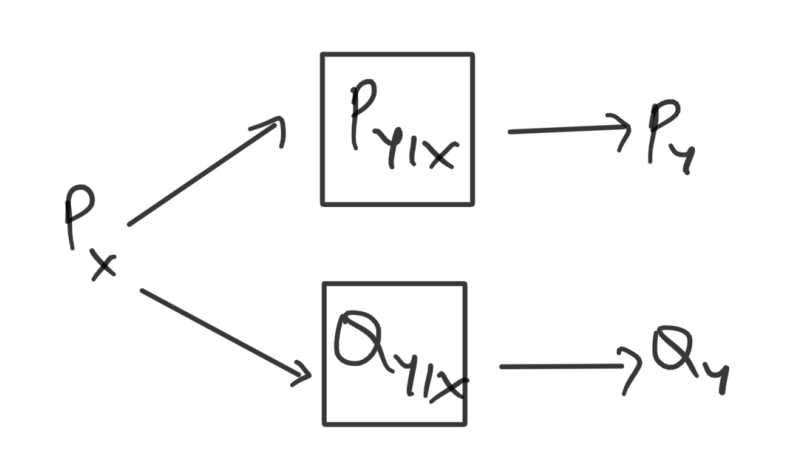
\includegraphics[width=0.3\linewidth]{Conditional_Divergence.png}
        \label{fig:Conditional_Divergence}
    \end{figure*}

    \noindent Then $\divergence{P_Y}{Q_Y}\le \divergence{P_\YgX}{Q_\YgX |P_X}$, with equality iff $\divergence{P_{X|Y}}{Q_{X|Y} |P_Y} = 0$.  
\end{theorem}

\begin{proof}
\begin{align*}
    \divergence{P_{X,Y}}{Q_{X,Y}}  &= \divergence{P_\YgX}{Q_\YgX |P_X} +  \underbrace{\divergence{P_X}{P_X}}_{ = 0} \\
        &= \underbrace{\divergence{P_{X|Y}}{Q_{X|Y} |P_Y}}_{\geq 0}  + \divergence{P_Y}{Q_Y}\\
    \implies \divergence{P_Y}{Q_Y} &\le \divergence{P_\YgX}{Q_\YgX |P_X}.
\end{align*}
\end{proof}

\begin{theorem}[DPI for Divergence]
    Given $P_\YgX, P_X$ and $Q_X$, let $P_Y = P_{Y|X} P_X$ and $Q_Y = P_{Y|X}Q_X$, as represented by the diagram. 
    \begin{figure*}[ht]
        \centering
        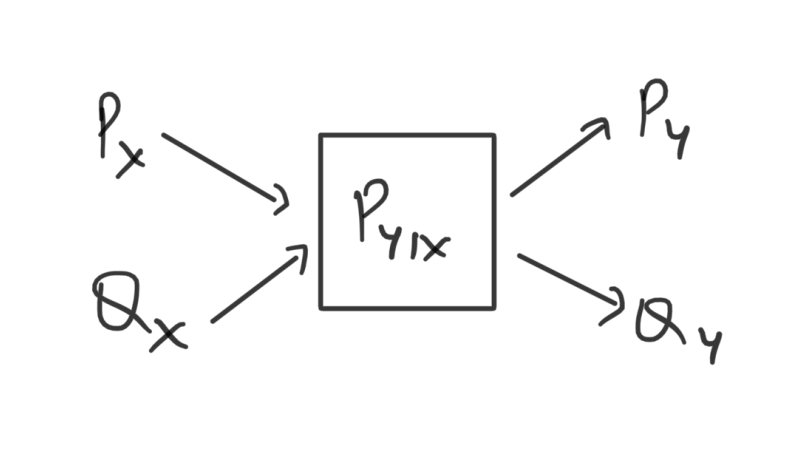
\includegraphics[width=0.3\linewidth]{DPI_Divergence.png}
        \label{fig:DPI_Divergence}
    \end{figure*}

    \noindent Then $\divergence{P_Y}{Q_Y}\le \divergence{P_X}{Q_X}$, with equality iff $\divergence{P_{X|Y}}{Q_{X|Y} |P_Y} = 0$.
\end{theorem}

\begin{proof}
    \begin{align*}
        \divergence{P_{X,Y}}{Q_{X,Y}}  &= \underbrace{\divergence{P_\YgX}{Q_\YgX |P_X}}_{=0} +  \divergence{P_X}{Q_X} \\
            &= \underbrace{\divergence{P_{X|Y}}{Q_{X|Y} |P_Y}}_{\geq 0}  + \divergence{P_Y}{Q_Y}\\
        \implies \divergence{P_Y}{Q_Y} &\le \divergence{P_X}{Q_X}.
    \end{align*}    
\end{proof}

\begin{theorem}
    DPI for Divergence implies DPI for Mutual Information.
\end{theorem}

\begin{proof}
    Now suppose we consider a Markov chain $X - Y - Z$ over discrete random variables. Then notice that 
    \begin{align*}
        P_{Z|X} = P_{Z|X,Y} P_{Y|X} {=} \textcolor{red}{P_{Z|Y}} P_{Y|X}, \quad P_Z = \textcolor{red}{P_{Z|Y}} P_Y.
    \end{align*}
    We apply DPI for divergence on $P_{Z|Y}, P_{Y|X=x}$ and $P_{Y}$ to get
    \begin{align}
        \divergence{P_{Y|X = x}}{P_{Y}}\ \ge \divergence{P_{Z|X = x}}{P_{Z}} \implies &\ \E_X \big[\divergence{P_{Y|X = x}}{P_{Y}}\big]\ \ge \E_X\big[\divergence{P_{Z|X = x}}{ P_{Z}}\big] \nonumber \\
        \implies &\ \divergence{P_{Y|X}}{P_{Y} | P_X}\ \ge \divergence{P_{Z|X}}{ P_{Z} | P_X}.\label{eqn:dpi}
    \end{align}
    Now consider the mutual information
    \begin{align*}
        I(X;Z) &= \divergence{P_{X,Z}}{P_X P_Z} \\
        &= \divergence{P_{Z|X}}{P_Z | P_X} \\
        &\le \divergence{P_{Y|X}}{P_Y | P_X},\qquad \text{(using \eqref{eqn:dpi})} \\
        &= \divergence{P_{X,Y}}{P_X P_Y} \\
        &= I(X; Y).
    \end{align*}
\end{proof}

\begin{theorem}[Golden Formula]
    \begin{align*}
        I(X;Y) = \min_{Q_{Y}} \divergence{P_{Y|X}}{Q_{Y}|P_{X}}.
    \end{align*}
\end{theorem}

\begin{proof}
    \begin{align*}
        \divergence{P_{Y|X}}{Q_{Y}|P_{X}} &= \divergence{P_{Y|X}P_{X}}{Q_{Y}P_{X}} \\ 
        &= \sum_{x,y} P_{X,Y} \log{\frac{P_{X,Y}}{Q_{Y}P_{X}} \frac{P_{Y}}{P_{Y}}} \\ 
        &= \sum_{x,y} P_{X,Y} \log{\frac{P_{X,Y}}{P_{X}P_{Y}} + \sum_{x,y} P_{X,Y} \log{\frac{P_{Y}}{Q_{Y}}}} \\ 
        &= \divergence{P_{X,Y}}{P_X P_Y} + \divergence{P_{Y}}{Q_Y} \\ 
        &= I(X;Y) + \divergence{P_{Y}}{Q_Y}.
    \end{align*}
    We get the result by noting that $D(P_{Y}||Q_{Y}) \ge 0$ where equality holds iff $Q_{Y} = P_{Y}.$        
\end{proof}

\begin{definition}
    Variational Distance.
\end{definition}

\begin{remark}
    Trivial bounds on variational distance.
\end{remark}

\begin{remark}
    Variational Distance is a Norm.
\end{remark}

\begin{theorem}
    Upper bound of relative entropy in terms of variational distance and entropy.
\end{theorem}

\begin{theorem}[Pinsker Inequality]

\end{theorem}

\begin{definition}
    Total Variation Distance.
\end{definition}

\section{Differential Entropy}

\section{Typicality}

\begin{definition}
    We say that a sequence of random variables $\{X_n\}$ \highlight{converges in probability} to a random variable $X$ if for all $\varepsilon > 0$, we have 
    \begin{equation*}
        \lim_{n\rightarrow \infty} \Prob\big[ |X_n - X| > \varepsilon \big] = 0.
    \end{equation*}
\end{definition}

\begin{lemma}[Markov Inequality]
    Let $X$ be a nonnegtaive random variable of finite mean $\E[X]<\infty$. Then for all $a>0$, we have
    \begin{equation*}
        \Prob[X\ge a] \le \dfrac{\E[X]}{a}.
    \end{equation*}
\end{lemma}

\begin{lemma}[Chebyshev Inequality]
    Let $X$ be a random variable with finite mean $\mu$ and finite variance $\sigma^2$. Then for all $\varepsilon>0$, we have
    \begin{equation*}
        \Prob[|X-\mu|\ge \varepsilon] \le \dfrac{\sigma^2}{\varepsilon}.
    \end{equation*}
\end{lemma}

\begin{lemma}[Weak Law of Large Numbers]
    Let $\{Z_n\}$ be a sequence of independent and identically distributed (i.i.d.) random variables with mean $\mu$ an variance $\sigma^2$. Let 
    \begin{equation*}
        S_n = \dfrac{1}{n}\sum_{k=1}^n Z_k
    \end{equation*}
    be the sample mean. Then $\{S_n\}$ converges in probability to $\mu$. In particular, 
    \begin{equation*}
        \Prob[|S_n-\mu|\ge \varepsilon] \le \dfrac{\sigma^2}{n\varepsilon^2}.
    \end{equation*}
\end{lemma}

\begin{definition}[Type]
    Let $x^{(n)}$ be a sequence of $n$ elements drawn from a finite-cardinality alphabet $\mathcal{X}$. The \highlight{empirical probability mass function} of $x^{(n)}$, also referred to as its \highlight{type}, is defined for $x\in \mathcal{X}$ as
    \begin{equation*}
        \pi(x|x^{(n)}) = \dfrac{|\{i\in [n]\;:\;x_i = x\}|}{n}, 
    \end{equation*}
    where $[n] = \{1,\ldots, n\}$.
\end{definition}

\begin{theorem}
    Let $\{X_n\}$ be an i.i.d.~sequence of random variables with $X_i\sim P_X(x_i)$. Then $\forall\ x\in\mathcal{X}$ and for all $\varepsilon>0$, we have
    \begin{equation*}
        \lim_{n\rightarrow 0} \Prob[|\pi(x|X^{(n)}) - P_X(x)| > \varepsilon] = 0, 
    \end{equation*}
    or in other words, $\{\pi(x|X^{(n)})\}$ converges in probability to $P_X(x)$ for all $x\in\mathcal{X}$.
\end{theorem}

\begin{definition}[Typical Set]
    The \highlight{set of $\varepsilon$-typical $n$-sequences} for a random variable $X\sim P_X$ and $\varepsilon \in (0,1)$ (simply typical set) is defined as
    \begin{equation*}
        \mathcal{T}^{(n)}_\varepsilon (X) = \{x^{(n)}\;:\; |\pi(x|x^{(n)}) - P_X(x)| \le \varepsilon P_X(x), \forall\ x\in\mathcal{X}\}.
    \end{equation*}
\end{definition}

\begin{remark}
    For an element $x\in\mathcal{X}$ which has $P_X(x)$ cannot be a part of typical sequence. Suppose such an $x$ belonged to a sequence $x^{(n)}$, then $\pi(x|x^{(n)}) > 0$. Consequently, we have $|\pi(x|x^{(n)}) - P_X(x)| = \pi(x|x^{(n)}) > 0 = \varepsilon P_X(x)$ for all $\varepsilon > 0$, which shows that $x^{(n)}$ is not a typical sequence.
\end{remark}

\begin{lemma}[Typical Average Lemma]
    Consider a typical sequence $x^{(n)}\in \mathcal{T}^{(n)}_\varepsilon (X)$. Then for any \highlight{nonnegtaive} function $g(\cdot)$ on $\mathcal{X}$, we have 
    \begin{equation*}
        (1-\varepsilon) \E[g(X)] \le \dfrac{1}{n} \sum_{k=1}^{n} g(x_k) \le (1+\varepsilon) \E[g(X)].
    \end{equation*}
\end{lemma}


\section{Source Coding}

\section{Joint Typical}

\begin{definition}[Joint Type]
    Let $(x^{(n)}, y^{(n)})$ be a sequence of a pair of $n$ length sequences from a finite-cardinality alphabet $(\mathcal{X},\mathcal{Y})$. The \highlight{joint empirical probability mass function} of $(x^{(n)}, y^{(n)})$, also referred to as its \highlight{joint type}, is defined for $x\in \mathcal{X}$ as
    \begin{equation*}
        \pi(x,y|x^{(n)}, y^{(n)}) = \dfrac{|\{i\in [n]\;:\;(x_i,y_i) = (x,y)\}|}{n}.
    \end{equation*}
\end{definition}

\begin{remark}
    The $X$-marginal of $X,Y$-joint empirical probability mass function is the $X$-empirical probability mass function.
\end{remark}

\begin{definition}[Jointly Typical Set]
    The \highlight{set of $\varepsilon$-jointly typical $n$-sequences} for a random variable $(X,Y)\sim (P_X,P_Y)$ and $\varepsilon \in (0,1)$ (simply jointly typical set) is defined as
    \begin{equation*}
        \mathcal{T}^{(n)}_\varepsilon (X,Y) = \{(x^{(n)},y^{(n)})\;:\; |\pi(x,y|x^{(n)},y^{(n)}) - P_{X,Y}(x,y)| \le \varepsilon P_{X,Y}(x,y), \forall\ x\in\mathcal{X}, y\in\mathcal{Y}\}.
    \end{equation*}
\end{definition}

\begin{remark}
    If $(x^{(n)},y^{(n)})\in \mathcal{T}_\varepsilon^{(n)}(X,Y)$, then $x^{(n)}\in \mathcal{T}_\varepsilon^{(n)}(X)$ and $y^{(n)}\in \mathcal{T}_\varepsilon^{(n)}(Y)$.
\end{remark}

\section{Channel Coding}

% \bibliographystyle{unsrt}
% \bibliography{ref}

\begin{thebibliography}{9}
    \bibitem{durisi21ssy210}
    Giuseppe Durisi. Lecture notes in SSY210-Information Theory, Chalmers University of Technology, 19th May 2021.

    \bibitem{moser2023information}
    Stefan M Moser. Information theory: Lecture notes (version 6.12 from 222 March 2023, PDF), 6th edition, ETH Z{ü}rich, 2023.

    \bibitem{cover2005elements}
    Thomas M. Cover and Joy A. Thomas. Elements of information theory, 2th edition. John Wiley \& Sons, 2005.

    % \bibitem{Rockafellar} 
    %     Rockafellar, R.T. Convex Analysis. Princeton University Press, 1972.
        
    % \bibitem{Fenchel}
    %     Fenchel, W. Convex Cones, Sets, and Functions. Princeton University, 1953.
\end{thebibliography}
        
    
\end{document}